\documentclass[conference]{IEEEtran}
\documentclass{article}
\IEEEoverridecommandlockouts
% The preceding line is only needed to identify funding in the first footnote. If that is unneeded, please comment it out.
\usepackage{cite}
\usepackage{amsmath,amssymb,amsfonts}
\usepackage{graphicx}
\usepackage{textcomp}
\usepackage{xcolor}
\usepackage{titlesec}
\usepackage{textcomp}
\usepackage{epsfig}
\usepackage{algpseudocode}
\usepackage{pgfplots}
\usepackage{tikz}
\usepackage{hyperref}
\usepackage{graphicx}
\usepackage{enumitem}
\usepackage[utf8]{inputenc}
\pgfplotsset{width=10cm,compat=1.9}
\usepgfplotslibrary{external}





\usepackage[linesnumbered,ruled,vlined]{algorithm2e}
\def\BibTeX{{\rm B\kern-.05em{\sc i\kern-.025em b}\kern-.08em
    T\kern-.1667em\lower.7ex\hbox{E}\kern-.125emX}}

\usepackage[ruled,vlined]{algorithm2e}

\tikzexternalize 
\begin{document}

\title{Implement Strassen’s Matrix Algorithm \\
\text{\Large{DAA ASSIGNMENT-4 , GROUP 6}}
}
\author{\IEEEauthorblockN{Shreyansh Patidar}
\IEEEauthorblockA{ \text{IIT2019018}}
\and
\IEEEauthorblockN{Biswajeet Das}
\IEEEauthorblockA{ \text{IIT2019019}}
\and
\IEEEauthorblockN{Hritik Sharma}
\IEEEauthorblockA{ \text{IIT2019020}}
}

\maketitle
{\textbf{\textit{Abstract:In this paper we have devised an algorithm which is an implementation of Strassen’s matrix algorithm using divide and
conquer.\\
\\This report further contains-
\begin{enumerate}[label=(\Roman*)]
    \item Algorithm Design 
    \item Algorithm Analysis 
    \item Result 
    \item Conclusion
\end{enumerate}
}}}
\maketitle

\section{INTRODUCTION}
In this report, we are going to discuss strassen matrix multiplication,formula of matrix multiplication and algorithms for strassen matrix multiplication.
Let us consider two matrices X and Y. We want to calculate the resultant matrix Z by multiplying X and Y. Matrix multiplication is a \href {https://en.wikipedia.org/wiki/Binary_operation}{binary operation} that produces a \href{https://en.wikipedia.org/wiki/Matrix_(mathematics)}{matrix} from two matrices. For matrix multiplication, the number of columns in the first matrix must be equal to the number of rows in the second matrix. The resulting matrix, known as the matrix product, has the number of rows of the first and the number of columns of the second matrix.
Thus the product XY is defined if and only if the number of columns in X equals the number of rows in Y.The utility of Strassen's formula is shown by its asymptotic superiority when order n of matrix reaches infinity.
\\\\ $Z = x_{i1}y_{1j}  + x_{i2}y_{2j} + …….+ x_{in}y_{nj} $ 
\\$Z = \Sigma x_{ik}y_{ki}$



\section{ALGORITHM DESIGN}
\\\\
\begin{enumerate}[label=(\Alph*)]
  \item Recursive method :
    \begin{enumerate}[label=(\arabic*)]
      \item Divide matrices A and B in 4 sub-matrices of
      \\ size n/2 X n/2.
      \item  Calculate following values Recursively.
      \\ae+bg , af+bh , ce + dg and cf+dh\\\\
    \end{enumerate}
\end{enumerate}


\graphicspath{ {./images/} }
\includegraphics[scale=0.60]{One}
\\A,B,C are square matrices of size nxn.
\\a,b,c,d are submatrices of A of size n/2 x n/2.
\\e,f,g,h are submatrices of size n/2 x n/2.
\\\\ In the above method , we do 8 multiplications for   
 matrices of n/2 x n/2 and 4 additions.\\

\renewcommand{\labelenumii}{\Alph{enumi}}
\begin{enumerate}[label=(\Alph*)]
  \setcounter{enumi}{1}
  \item Strassen’s Algorithm \\
\end{enumerate}

The Strassen’s method of matrix multiplication is a typical divide and conquer algorithm
The idea of Strassen’s method is to reduce the number of recursive calls to 7.\\
Strassen’s method is similar to above simple divide and conquer method in the sense that this method also divide matrices to sub-matrices of size N/2 x N/2 , but in Strassen’s method, the four sub-matrices of result are calculated using following formulae.\\\\
P1 = a(f-h)     P2 = (a+b)h    P3 = (c+d)e\\
P4 = d(g-e)    P5 = (a+d)(e+h)   P6 = (b-d)(g+h)\\
P7 = (a-c)(e+f)\\\\

\graphicspath{ {./images/} }
\includegraphics[scale=0.70]{Two}\\\\
C11 = p5 + p4 - p2 + p6\hspace{1cm}       C12 = p1 + p2\\
C21 = p3 + p4\hspace{1cm}     C22 = p1 + p5 - p3 - p7\\\\


\\\\Here we describe 2 possible approaches :\\\\
{\textbf{Approach 1:}} \\\\
This is a brute force approach for multiplication of two matrices.\\
Simply run three loops. Loop for each row in matrix A with variable i.Inside the above loop, Loop for each column in matrix B with variable j. Inside the above two loops, Loop for each row element in matrix A with variable k and each column element in matrix B with variable k  ie, A[i][k] and B[k][j].
we will find the product of each row element in A with each column element in B. ie, A[i][k] * B[k][j] and add all the products and store in the new matrix C ie, C[i][j]. matrix C is the multiplication output.\\\\

{\textbf{Approach 2:}} \\\\
Divide a matrix of order of n*n recursively till we get the matrix of 2*2.Use the previous set of formulas to carry out 2*2 matrix multiplication.In this eight multiplication and four additions, subtraction is performed.Combine the result of two matrices to find the final product or final matrix.\\\\

{\textbf{Algorithm 1:}} \\\\
\begin{algorithm}[H] 
    \caption{Matrix-Multiplication (X, Y, Z)}
    \DontPrintSemicolon
    \SetKwFunction{FMain}{Main}
    \SetKwProg{Fn}{Function}{:}{}
    \Fn{\FMain{}}{
    
    if
    
    \For{$i \gets 1$ \textbf{ to } $p$} 
          {
            \For{$j \gets 1$ \textbf{ to } $r$}
              {
                $Z[i,j]$ = $0$
                 \For{$k \gets 1$ \textbf{ to } $q$}
              {
                $Z[i,j]$ = $Z[i,j]$ + $X[i,k]$ × $Y[k,j]$

              }
              }
                
            
              
         }
                

 }\\\\\\
\end{algorithm}

{\textbf{\\\\Algorithm 2:}} \\\\
\begin{algorithm}[H] 
    \caption{Strassen’s Algorithm }
    \DontPrintSemicolon
    \SetKwFunction{FMain}{Strassen(n, a, b, d)}
    \SetKwProg{Fn}{Function}{:}{}
    \Fn{\FMain{}}{
    
    \eIf{ n = 1}{
   return A_{11}B_{11}\;
   
   }{
   Partition a into four sub matrices  a11, a12, a21, a22.\;
   Partition b into four sub matrices b11, b12, b21, b22.\;
  }
  
   Strassen ( n/2, a11 + a22, b11 + b22, d1)\\
	Strassen ( n/2, a21 + a22, b11, d2)\\
	Strassen ( n/2, a11, b12 – b22, d3)\\
	Strassen ( n/2, a22, b21 – b11, d4)\\
	Strassen ( n/2, a11 + a12, b22, d5)\\
	Strassen (n/2, a21 – a11, b11 + b22, d6)\\
	Strassen (n/2, a12 – a22, b21 + b22, d7)\\
	
	C = d1+d4-d5+d7\hspace{1cm} d3+d5\\
	   \hspace{1cm}d2+d4\hspace{1cm}           d1+d3-d2-d6  
	
	return (C)
	
}
\end{algorithm}
\hfill \break


\section{ALGORITHM AND ANALYSIS\\}
\begin{enumerate}[label=(\Alph*)]
  \item \\Time Complexity  :\\
\end{enumerate}

{\textbf{Approach 1:}} \\\\
 Here, we assume that integer operations take O(1) time. Here we simply run three loops first loop run r1  times, the second loop runs c2 times, and  the final loop runs r2 times.\\
$t_{avg}$ = $O(n*n*n)$\\
$t_{best}$ = $O(0)$\\

{\textbf{Approach 2:}} \\\\
Addition and Subtraction of two matrices takes $O(N^2)$ time. So time complexity can be written as:\\
$T(N)$ = $7T(N/2) +  O(N^2)$\\
From Master's Theorem, time complexity of  
above method is $O(N^{Log7})$\\\\
$t_{avg}$ = $O(N^{Log7})$ \\
$t_{best}$ = $O(0)$\\

\renewcommand{\labelenumii}{\Alph{enumi}}
\begin{enumerate}[label=(\Alph*)]
  \setcounter{enumi}{1}
  \item  Space Complexity
\end{enumerate}
\\The space complexity of this algorithm for both the approaches are as follows:\\

{\textbf{Approach 1:}} \\\\
Here we create extra space for storing the result of the multiplication of matrices. Here we also declared r1*c1 size for taking input the first matrix and r2*c2 size for taking input the second Matrix.\\
Space complexity : $O(n^2)$ \\

{\textbf{Approach 2:}} \\\\
Computing S1, . . . , S7 and the matrix that we return in the last step requires $O(n^2 )$ space.We start with $3n^2$ space for the two input matrices and the output matrix. We then allocate $3(n/2)^2$ space for the recursive call to compute S1. Once S1 is returned, we add it to the upper left quadrant of the output matrix. In this same $3(n/2)^2$ space, we compute S2, and then we add it to the upper left and lower right quadrants of the output matrix. We continue in the same manner for the rest of the $S_i$\\
Space complexity :  $O(n^2)$     \\



\section{Experimental Analysis}


\textbf{Graph - 1 : } it can be clearly seen that first graph has $O(n^3)$ behaviour.

\textbf{Graph - 2 : } it can be clearly seen that first graph has something like $n^2$ behaviour.


\begin{flushleft}

\begin{tikzpicture}
\begin{axis}[
    title={n vs t graph for algorithm - 1},
    xlabel={Dimension [n]},
    ylabel={Time [t in ns]},
    xmin=0, xmax=50,
    ymin=0, ymax=80000,
    xtick={0,10,20,30,40},
    ytick={0,10000,20000,30000,40000,50000,60000,70000}
]
\addplot[
    color=red,
    mark=dot,
    ]
    coordinates {
   (0,0)(5,120)(10,1010)(15,3365)(19,6851)(24,13874)(29,24399)(30,27023)(32,32758)(45,91168)
    };
    
  \end{axis}
  


\end{tikzpicture}
\end{flushleft}


\begin{flushleft}

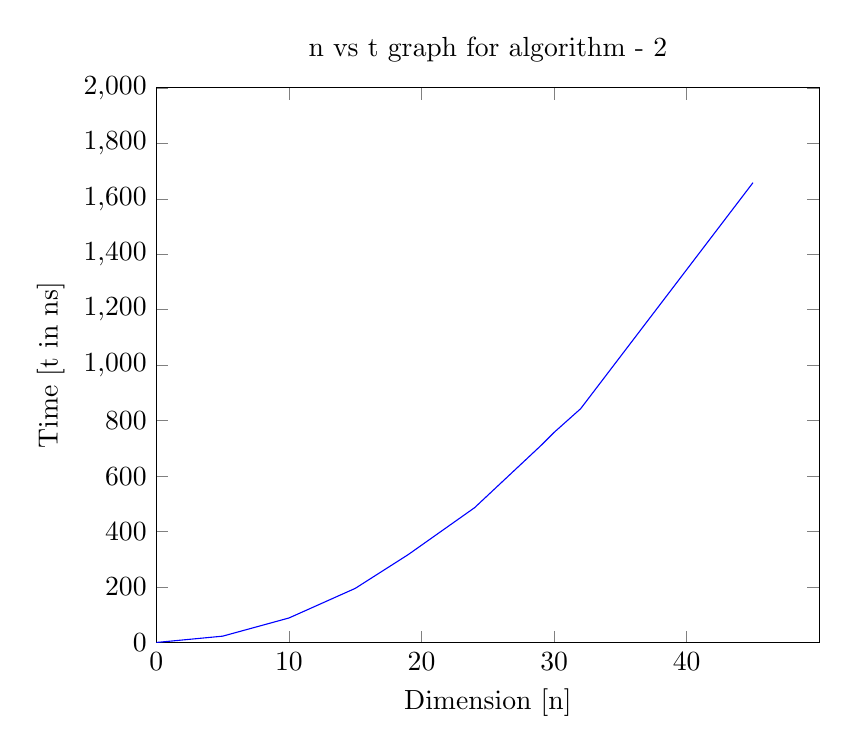
\begin{tikzpicture}
\begin{axis}[
    title={n vs t graph for algorithm - 2},
    xlabel={Dimension [n]},
    ylabel={Time [t in ns]},
    xmin=0, xmax=50,
    ymin=0, ymax=2000,
    xtick={0,10,20,30,40},
    ytick={0,200,400,600,800,1000,1200,1400,1600,1800,2000}
]
\addplot[
    color=blue,
    mark=dot,
    ]
    coordinates {
  (0,0)(5,22.81)(10,88.35)(15,195.12)(19,317.05)(24,486.02)(29,709.93)(30,757.64)(32,842.93)(45,1658.07)
    };
    
  \end{axis}
  


\end{tikzpicture}
\end{flushleft}


\section{CONCLUSION\\}
Implementation of Strassen's algorithm for matrix multiplication is several times faster than the naïve method for matrix multiplication, if applied on large enough matrices.\\

\section{REFERENCES\\}
\begin{enumerate}
    \item \url{https://www.geeksforgeeks.org/strassens-matrix-multiplication/}
    \item \url{https://www.cs.cmu.edu/~15451-f19/LectureNotes/lec01-strassen.pdf}
\end{enumerate}
\end{document}
